% !TeX spellcheck = en_US
\documentclass[french]{yLectureNote}

\title{Introduction à la termodynamique}
\subtitle{Thermodynamique}
\author{Paulhenry Saux}
\date{\today}
\yLanguage{Français}

\professor{}

\usepackage{graphicx}%-pour mettre des images
\usepackage[utf8]{inputenc}%encodage
\usepackage{geometry}%pour modifier les tailles et mettre a4paper
%\usepackage{awesomebox}%pour les boites d'exercices, de pbq et de croquis d\'esactiv\'e pour les TP de PC
\usepackage{tikz}%pour deiffner + d\'ependance de chemfig
\usepackage{tkz-tab}
\usepackage{tabularx}%pour dimensionner automatiquement les tableaux avec variable X
\usepackage{awesomebox}%Pour les boites info, danger et autres
\usepackage{menukeys}%Pour deiffner les touches de Calculatrice
\usepackage{fancyhdr}%pour les en-t\^ete personnalis\'ees
\usepackage{blindtext}%pour les liens
\usepackage{hyperref}%pour les liens (\`a mettre en dernier)
\usepackage{caption}%pour la francisation de la l\'egende table vers Tableau
\usepackage{pifont}
\usepackage{array}%pour les tableaux
\usepackage{lipsum}
\usepackage{yFlatTable}
\usepackage{multicol}
\newcommand{\Lim}[1]{\lim\limits_{\substack{#1}}\:}
\renewcommand{\vec}{\overrightarrow}
\newcommand{\bz}{\overline{z}}
\DeclareMathOperator{\card}{card}
\renewcommand{\vec}{\overrightarrow}
\newcommand{\N}[0]{\mathbb{N}}
\newcommand{\R}[0]{\mathbb{R}}
\newcommand{\C}[0]{\mathbb{C}}
\newcommand{\dd}[0]{\mathrm{d}}
\newcommand{\er}{\vec{e_{\rho}}}
\newcommand{\ep}{\vec{e_{\varphi}}}
\newcommand{\pip}{\pi^+}
\newcommand{\pim}{\pi^-}
\newcommand{\mv}{\mathcal{V}}
\DeclareMathOperator{\Div}{Div}
\newcommand{\rot}{\vec{\mathrm{rot}}}
\newcommand{\grad}{\vec{\mathrm{grad}}}
\begin{document}
\setcounter{chapter}{5}

\chapter{Transition de phase : Corps homogène}

\section{Analyse}
% Page 1 (P21) : Introduction à la Partie 2
\subsection{Stabilité de l'équilibre du corps homogène}

\checkInfo{Objet de l'étude}{Analyse de la stabilité pour une phase unique : solide, liquide ou vapeur.}



% Pages 2-3 (P22-P23) : Mise en œuvre et Point de départ
\subsection{Méthodologie d'analyse}

\checkInfo{Objectif}{Déterminer si le système reste dans une phase donnée (liquide ou vapeur) lorsqu'il est au contact d'une atmosphère à $T$ et $P$ fixées.}


L'analyse repose sur l'utilisation du potentiel thermodynamique $G$ (Enthalpie libre)\marginInfo{On choisit $G$ car dans la majorité des expériences de transition de phase, l'expérimentateur contrôle la pression $P$ (poids) et la température $T$ (thermostat).}.


%\tipsInfo{Modèles phénoménologiques}{On utilise les modèles de Gaz Parfait et de Liquide/Solide pour exprimer les isothermes $P(v)$.}



% Pages 4-5 (P24-P25) : Expression de $G$ pour le Gaz Parfait
\subsection{Potentiel $G$ du Gaz Parfait}

\begin{definition}
Pour un gaz parfait à température $T_0$, l'enthalpie libre molaire s'exprime en fonction de la pression $P$ :
$$g_{GP}(T_0, P) = g^\circ(T_0) + RT_0 \ln\left(\frac{P}{P^\circ}\right)$$.
\end{definition}

%\checkInfo{Comportement}{La fonction $g(P)$ est une fonction croissante et concave (sa pente diminue quand $P$ augmente).}



% Pages 6-8 (P26-P28) : Expression de $G$ pour la phase Condensée
\subsection{Potentiel $G$ du Liquide et du Solide}

\begin{proposition}
Pour une phase condensée (liquide ou solide) considérée comme incompressible et indilatable ($v \approx \text{cste}$) :
$$g_{liq}(T_0, P) = g_{liq}(T_0, P_{ref}) + v_{liq}(P - P_{ref})$$.
\end{proposition}

\warningInfo{Linéarité}{Contrairement au gaz, l'évolution de $G$ avec la pression est ici linéaire car le volume molaire $v$ est quasiment constant.}



% Page 9 (P29) : Cas de la phase Solide
\subsection{Spécificités du Solide}

\checkInfo{Modèle}{Le solide est traité comme une phase incompressible avec un volume molaire $v_s < v_l$ (cas général hors eau).}

% \begin{proposition}
% L'expression est identique au liquide : $G_{T_0,s}(P) = v_s P + \text{cte}$.
% \end{proposition}



% Page 10 (P30) : Comparaison des Potentiels
\subsection{Hiérarchisation des stabilités}

\criticalInfo{Critère de sélection}{À $T$ et $P$ données, la phase physiquement réalisée est celle qui possède l'enthalpie libre $G$ la plus faible.}





% Pages 11-13 (P31-P33) : Application du critère de Gibbs-Duhem
\subsection{Stabilité intrinsèque}

\begin{theorem}
Un état d'équilibre d'un corps homogène est intrinsèquement stable si :
$$\left( \frac{\partial P}{\partial V} \right)_T \le 0$$.
\end{theorem}

\checkInfo{Interprétation}{Cela signifie que le coefficient de compressibilité isotherme $\chi_T$ doit être positif. Une augmentation de pression doit entraîner une diminution de volume.}



% Pages 14-15 (P34-P35) : Pression de Saturation
% \subsection{Équilibre de Coexistence}

% \begin{definition}
% La pression de saturation $P_{sat}(T_0)$ est la pression pour laquelle les potentiels chimiques des deux phases sont égaux :
% $$g_{liq}(T_0, P_{sat}) = g_{vap}(T_0, P_{sat})$$.
% \end{definition}

% \tipsInfo{Intersection}{Graphiquement, c'est le point où les courbes $g(P)$ du liquide et de la vapeur se croisent.}

\subsection{Représentations graphiques}




\criticalInfo{Transition}{À $P = P_{sat}$, le système peut exister sous les deux formes ; c'est le début du changement d'état.}
\section{Résultats}
\subsection{Diagrammes à connaître}
\subsubsection{Diagramme G et P + V et P}

\includegraphics[scale=0.5]{c2}
\subsubsection{Diagramme P et T}
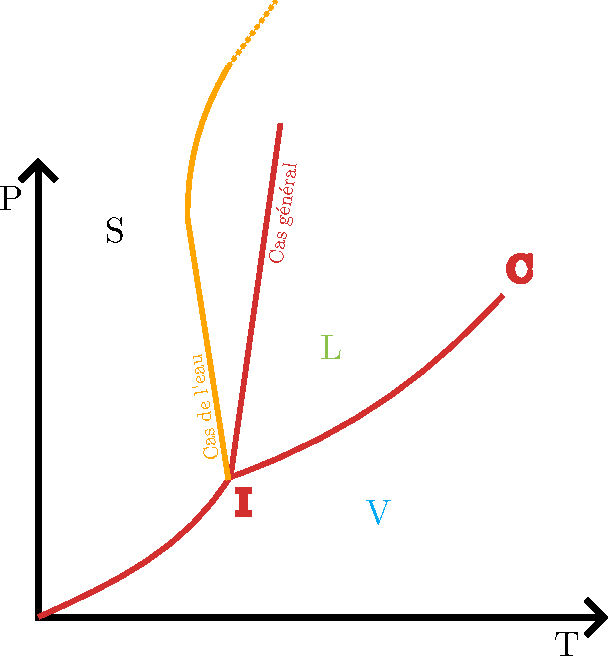
\includegraphics[scale=0.5]{dpt}
\subsection{Chaleur latente}
\begin{definition}[Chaleur latente]
    $$l_v(T) = h_v(T)^{Sat}-h_L(T)^{Sat}$$ avec $h = H/m$ ou $h=H/n$.
\end{definition}
\begin{theorem}[Relation de Clapeyron]
    $$l_v(T) = T(v_v^{Sat}-v_L^{Sat})\frac{\dd p_{sat}}{\dd T}$$
\end{theorem}
Cette relation permet d'obtenir des informations sur une grandeur énergétique à partir de la connaissance des conditions de saturation (pression de saturation et des volumes de saturation).
\begin{theorem}[Expression des enthalpies pour un changement de phase]
    $$H_v-H_L = H_v-H_v^{Sat}+ml_v(T_s)+H_L-H_L$$
\end{theorem}
\end{document}


